\section{Figures} \label{sectionExample}

Figure~\ref{ExampleEstNoiseCovar}, is an example of a figure with a legend.

\begin{figure}[h]
\centering
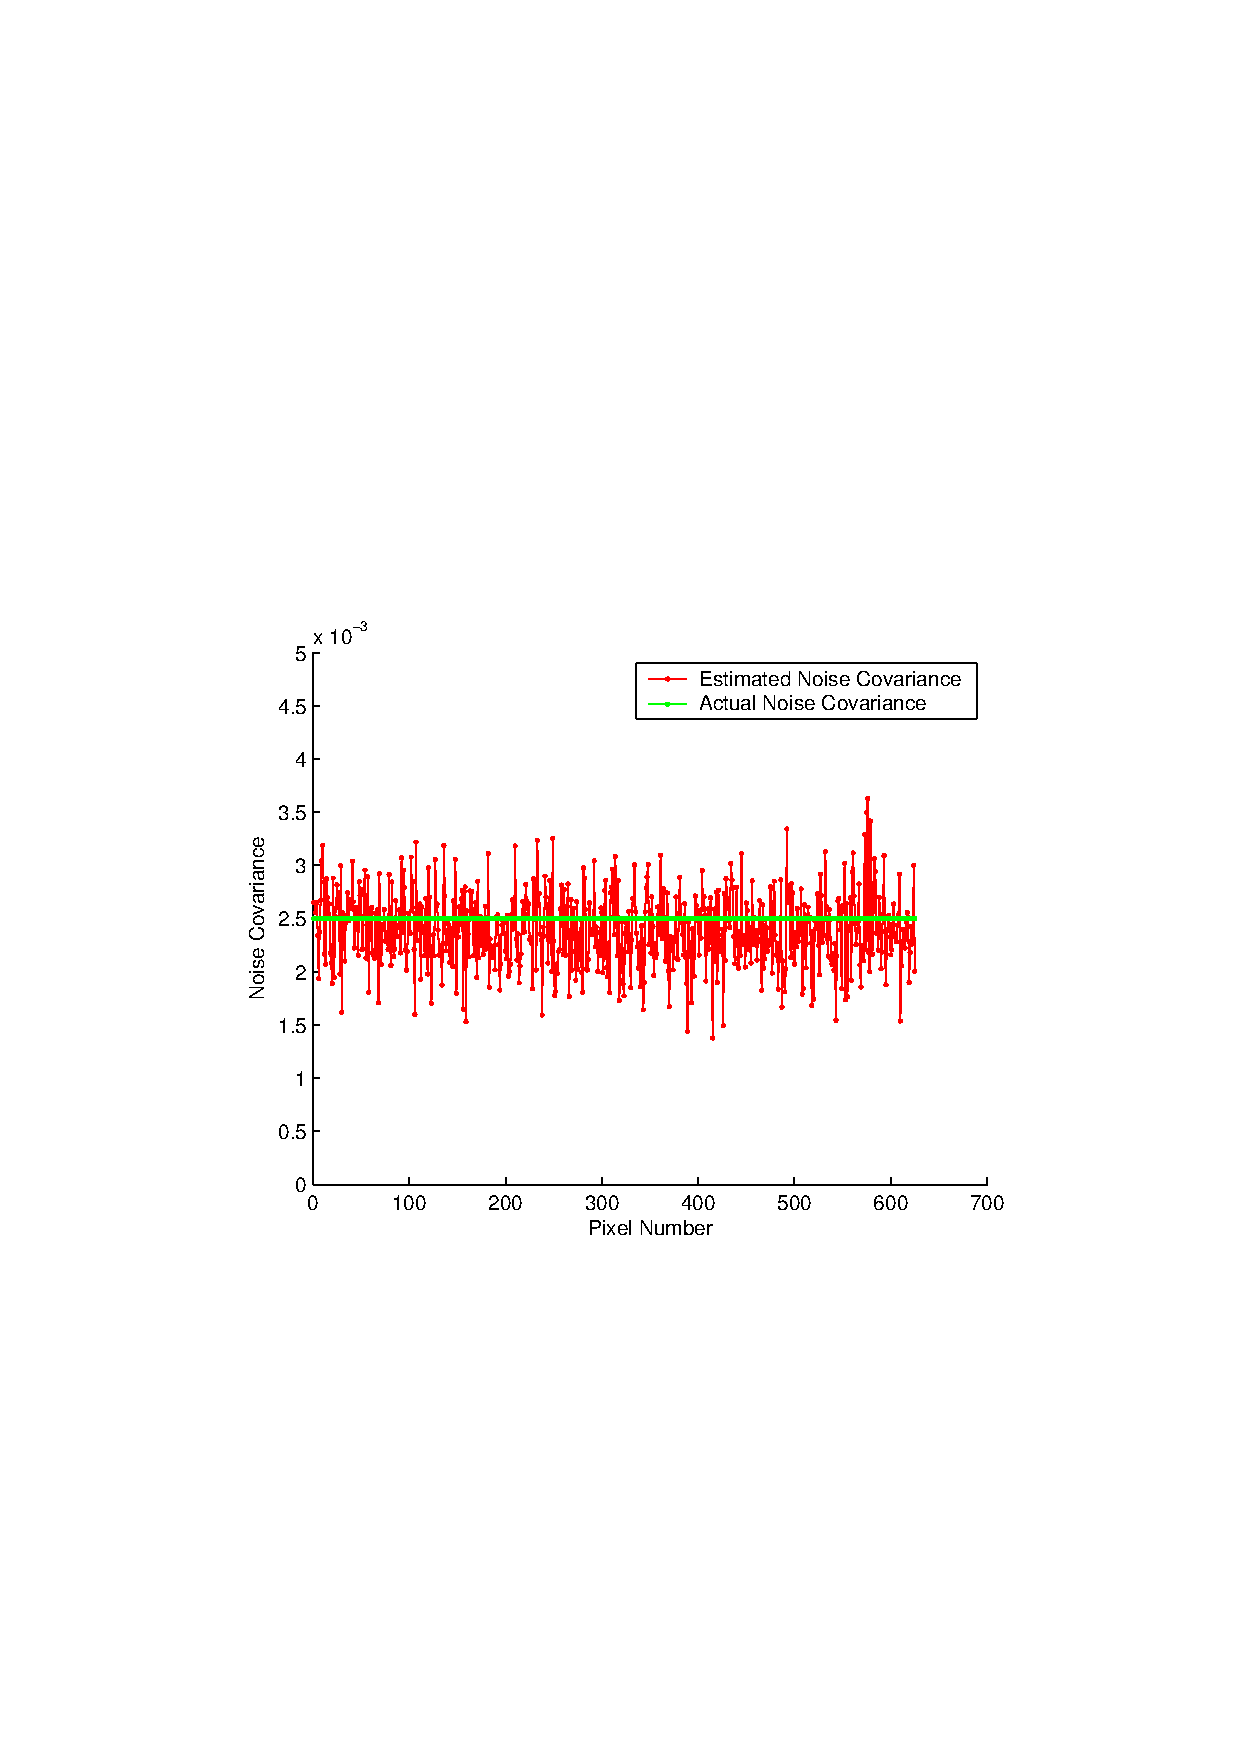
\includegraphics[width=0.5\linewidth]{exampleEstNoiseCovar}
\caption{This is the figure caption. Notice the figure looks good even when magnified because it is a vector-graphic, and not rasterized.} \label{ExampleEstNoiseCovar}
\end{figure}


\textbf{Old and New Instructions} These instructions are partly ``old'' because instead of .eps, we usually put pdf or png figures in our documents these days. However, they're still useful because exporting of Matlab figures directly to pdf, when using the Student License version of Matlab, results in an undesirable watermark. So my advice is to prepare your raster images as .png's, prepare your vector graphics as .pdf's in Inkscape or even Office (with the MS plugin that exports to .pdf), and follow the following slightly roundabout process to get Matlab figures into .pdf form.
\begin{enumerate}
  \item Make the figure in Matlab.
  \item Do \texttt{print -depsc2} to generate an .eps.
  \item Open the .eps in Ghostview (GSview) and ``Convert'' using the ``pdfwrite'' device to save a .pdf.
\end{enumerate}



\section{Test plan} \label{sec:test}

In the early stage, testing and verification of the algorithms and retrieval system are vital. While the retrieval system is completed, some test cases are also important to evaluate the performance of the system. A series of tests are carried out:

\begin{enumerate}[1)]
\item Retrieval test
\item Rotation invariant test
\item Noise invariant test
\item ``Scan to search'' test
\item Large database test
\end{enumerate}

The first step is to test that the retrieval system can operate correctly. A model from the model database will be input to the search engine to retrieve. The result is expected to find the model which is exact the same as the input one. 

The second step is to verify the descriptors are correctly computed, i.e., the rotational invariance property of the descriptors is shown. A model from the model database will be loaded, and a random rotation will be applied to the model. Then this model is queried in the system. The best result is finding out exact the same model from the database. However, due to the protential error of coefficients in rotation or rasterization, if the system shows models with similar shape, the system can still be decided as robust. 

The third step is to test the denoising module and verify the noise resistant property of the system. A model from the model database will be loaded and noise will be added. Then the denoising function is called. As the denoise module and the rasterization module cannot perfectly eliminate the noise, the system can be decided as robust if the query result shows models with same or similar shapes. 

If the first three tests are passed, the pre-processing modules and the matching algorithm are considered to be correctly implemented. Afterwards, ``Scan to search'' test can be carried out. The scanned model is loaded and denoised. Then the model is queried in the system. The results will indicate how well the matching algorithm works. The last test is to verify the system's robustness to large database, where a large number of descriptors may have influence to the retrieval accuracy. 

\section{Results} \label{sec:results}

\begin{enumerate}
\item Retrieval test

The aim of this test is to make sure the retrieval system can operate successfully. As Figure~\ref{retrievaltest_UI} demonstrates, the test result indicates every module of the retrieval system is correctly implemented, and the models in the database can be retrieved. 

\begin{figure}
\begin{center}
\begin{tabular}{cc}   % The "|" bar puts a bar in the figure
   \includegraphics[width=0.6\linewidth]{input_initialdesign}  \\
   (a) \\
\end{tabular}
   \includegraphics[width=1\linewidth]{output_finaldesign}  \\
   (b)  \\
\caption{Retrieval test: the input model is in (a) and the query results are in (b). The results indicate every module of the retrieval system is correctly implemented, and the models in the database can be retrieved successfully} 
  \label{retrievaltest_UI}
\end{center}
\end{figure}

\item Rotation invariant test

There are two test cases in this test. The first is to input a rotated model with a cylinder-like shape and search. The input and output are demonstrated in Figure~\ref{noiseinvarianttest_UI1}.  It can be noitced that the first candidate model (with the highest similarity) has exactly the same shape as the input model. Two types of descriptors of the rotated model and the matched model are analised and plotted(Figure~\ref{rotationinvarianttest_analysis1}). Comparing with the rotated model and the origin model, their spherical harmonics descriptors have almost the same feature in 2D, and their distance histogram descriptors have almost the same feature in 1D. Thus the rotation invariant property of the two descriptors is verified.

\begin{figure}
\begin{center}
\begin{tabular}{cc}   % The "|" bar puts a bar in the figure
   \includegraphics[width=0.6\linewidth]{input_rotationinvariant_test10}  \\
   (a) \\
\end{tabular}
   \includegraphics[width=1\linewidth]{output_rotationinvariant_test10}  \\
   (b)  \\
\caption{Rotation invariant test 1: the input model is in (a) and the query results are in (b). It can be noitced that the first candidate model has the same shape as the input model.} 
  \label{noiseinvarianttest_UI1}
\end{center}
\end{figure}

\begin{figure}
\begin{center}
\begin{tabular}{cc}   % The "|" bar puts a bar in the figure
   \includegraphics[width=0.45\linewidth]{rotationinvariant_test_SH10_rotated} & 
   \includegraphics[width=0.45\linewidth]{rotationinvariant_test_SH10_origin}  \\
   (a) Spherical harmonics (rotated model) & (b) Spherical harmonics (origin model) \\
   \includegraphics[width=0.45\linewidth]{rotationinvariant_test_DH10_rotated} &
   \includegraphics[width=0.45\linewidth]{rotationinvariant_test_DH10_origin}  \\
   (c) Distance histogram (rotated model) & (d) Distance histogram (origin model)\\
\end{tabular}
\caption{Analysis of the rotation invariant test 1: (a) and (b) have almost the same statistical distribution, (c) and (d) have almost the same statistical distribution. Thus the rotation invariant property of the two descriptors is verified.} 
  \label{rotationinvarianttest_analysis1}
\end{center}
\end{figure}

In the second test, a flat model is rotated and queried. This is to test the robustness of the descriptors against any rotated shape. Figure~\ref{noiseinvarianttest_UI2} demonstrates the input and output. Also, the same model is found. However, the analysis of the descriptors (Figure~\ref{rotationinvarianttest_analysis2}) shows that there is an unusual burst in the spherical harmonics descriptors of the rotated model(located in radius range 12 to 13). It is perhaps caused by the sampling error in rasterization. But with the assistance of the distance histogram descriptors, whose statistical feature almost have no difference in this case, the final matching result is still satisfactory. 

\begin{figure}
\begin{center}
\begin{tabular}{cc}   % The "|" bar puts a bar in the figure
   \includegraphics[width=0.6\linewidth]{input_rotationinvariant_test32}  \\
   (a) \\
\end{tabular}
   \includegraphics[width=1\linewidth]{output_rotationinvariant_test32}  \\
   (b)  \\
\caption{Rotation invariant test 2: the input model is in (a) and the query results are in (b). It can be noitced that the first candidate model has the same shape as the input model.} 
  \label{noiseinvarianttest_UI2}
\end{center}
\end{figure}

\begin{figure}
\begin{center}
\begin{tabular}{cc}   % The "|" bar puts a bar in the figure
   \includegraphics[width=0.45\linewidth]{rotationinvariant_test_SH32_rotated} & 
   \includegraphics[width=0.45\linewidth]{rotationinvariant_test_SH32_origin}  \\
   (a) Spherical harmonics (rotated model) & (b) Spherical harmonics (origin model) \\
   \includegraphics[width=0.45\linewidth]{rotationinvariant_test_DH32_rotated} &
   \includegraphics[width=0.45\linewidth]{rotationinvariant_test_DH32_origin}  \\
   (c) Distance histogram (rotated model) & (d) Distance histogram (origin model)  \\
\end{tabular}
\caption{Analysis of the rotation invariant test 2: Comparing with (a) and (b), there is an unusual burst in (a) (located in radius range 12 to 13). It is perhaps caused by the sampling error in rasterization. 
With the assistance of (c), whose statistical feature almost have no difference with (d), the final matching result is still satisfactory.} 
  \label{rotationinvarianttest_analysis2}
\end{center}
\end{figure}


\item Noise invariant test

INPUT UI
OUTPUT UI

\begin{figure}
\begin{center}
\begin{tabular}{cc}   % The "|" bar puts a bar in the figure
   \includegraphics[width=0.45\linewidth]{input_noiseinvariant_test_addnoise10} & 
   \includegraphics[width=0.45\linewidth]{input_noiseinvariant_test_denoise10}  \\
   (a) & (b) \\
\end{tabular}
   \includegraphics[width=1\linewidth]{output_noiseinvariant_test10}  \\
   (c)  \\
\caption{Another figure caption. These should be meaningful and somewhat self-contained.} 
  \label{noiseinvarianttest_UI}
\end{center}
\end{figure}

SH  DH   vs SH DH

\begin{figure}
\begin{center}
\begin{tabular}{cc}   % The "|" bar puts a bar in the figure
   \includegraphics[width=0.45\linewidth]{noiseinvariant_test_SH10_denoise} & 
   \includegraphics[width=0.45\linewidth]{noiseinvariant_test_SH10_origin}  \\
   (a)denoise & (b)origin                                                     \\
   \includegraphics[width=0.45\linewidth]{noiseinvariant_test_DH10_denoise} &
   \includegraphics[width=0.45\linewidth]{noiseinvariant_test_DH10_origin}  \\
   (c)denoise & (d) origin                                                    \\
\end{tabular}
\caption{Another figure caption. These should be meaningful and somewhat self-contained.} 
  \label{noiseinvarianttest_analysis}
\end{center}
\end{figure}


``Scan to search'' test 
INPUT UI
OUTPUT UI

\begin{figure}
\begin{center}
\begin{tabular}{cc}   % The "|" bar puts a bar in the figure
   \includegraphics[width=0.6\linewidth]{input_scantosearch_test}  \\
   (a) \\
\end{tabular}
   \includegraphics[width=1\linewidth]{output_scantosearch_test}  \\
   (b)  \\
\caption{Another figure caption. These should be meaningful and somewhat self-contained.} 
  \label{scantosearchtest_UI}
\end{center}
\end{figure}


SH  DH   vs   SH DH

\begin{figure}
\begin{center}
\begin{tabular}{cc}   % The "|" bar puts a bar in the figure
   \includegraphics[width=0.45\linewidth]{scantosearch_test_SH_scanned} & 
   \includegraphics[width=0.45\linewidth]{scantosearch_test_SH_matched}  \\
   (a)denoise & (b)origin                                                     \\
   \includegraphics[width=0.45\linewidth]{scantosearch_test_DH_scanned} &
   \includegraphics[width=0.45\linewidth]{scantosearch_test_DH_matched}  \\
   (c)denoise & (d) origin                                                    \\
\end{tabular}
\caption{Another figure caption. These should be meaningful and somewhat self-contained.} 
  \label{scantosearchtest_analysis}
\end{center}
\end{figure}

Large database test
NO FIGURES
In the initial design, there is only one spherical harmonics descriptors. And a single type of descriptors may have its weakness. Due to some unknown errors in the descriptors (maybe it is the rasterization error or sampling error in the spherical harmonics transformation), there are sometimes some irrelevant matches. This is analysed in Section~\ref{sec:thefinaldesign}.  Also as test result suggests, another type of descriptors (distance histogram) is added for assistance. 

\end{enumerate}

%example for subfigure
%\begin{figure}
%    \begin{subfigure}[b]{.45\linewidth}
%        \centering
%            \includegraphics[scale=.3]{rotationinvariant_test_SH10}
%            \caption{Skeletal}
%        \label{fig:SkeletalTissue}
%    \end{subfigure}
%    \begin{subfigure}[b]{.45\linewidth}
%        \centering
%            \includegraphics[scale=.3]{rotationinvariant_test_SH10}
%            \caption{Cardiac}
%        \label{fig:CardiacTissue}
%    \end{subfigure}
%    \caption{Types of Muscular Tissue}
%    \label{fig:MuscularTissue}
%\end{figure}